\section{Módulo vectorial: IVF en disco y planificador híbrido}
\label{sec:vectorial}

% ---------------------------------------------------------------------------
% ROL 3: primera versión redactada por el Rol 4 a partir del README y de
% benchmarks/results/exp8_*.csv para que el informe compile completo. Ajusta lo
% que haga falta (sobre todo el análisis del 8b y los diagramas).
% ---------------------------------------------------------------------------

\subsection{El tipo \code{VECTOR(D)} y la búsqueda exacta}

Un \code{VECTOR(D)} son $D$ \code{float32} contiguos ($4D$ bytes), así que sigue siendo
un tipo de ancho fijo y toda la maquinaria de páginas, bitmap y RID del Proyecto 1 se
aplica sin cambios. Las distancias soportadas son L2 (\code{<->}) y coseno
$1-\cos\theta$ (\code{<=>}). La línea base es el k-NN lineal
(\code{backend/vector/knn.py}): recorre la tabla por lotes, calcula las distancias con
\code{numpy} y mantiene los $k$ mejores en un Max-Heap de tamaño $k$, de modo que un
candidato nuevo se compara con la raíz en $O(1)$ y entra en $O(\log k)$. Es la verdad
de campo del Experimento 8 y la ruta \code{KnnSeqScan} del planificador.

\subsection{Diseño en disco del IVF}

El espacio se parte en $C=\lfloor\sqrt{N}\rfloor$ celdas de Voronoi con K-Means++
(esférico cuando la métrica es coseno). Dos archivos paginados:

\begin{table}[H]
\centering\small
\begin{tabularx}{\textwidth}{llY}
\toprule
Archivo & Registro & Metadatos \\
\midrule
\code{<t>\_\_<idx>.ivf.dir} & $\langle$centroide \code{VECTOR(D)}, cluster\_id, head, tail, count$\rangle$ & \code{user\_a} = métrica, \code{user\_b} = $C$ \\
\code{<t>\_\_<idx>.ivf.lst} & $\langle$pk, page, slot, area, vec$\rangle$, una cadena de páginas por celda & \code{user\_a} = $N$ \\
\bottomrule
\end{tabularx}
\end{table}

Las listas son densas y una página se decodifica de una vez con
\code{numpy.frombuffer}. Se guarda la clave primaria junto al RID porque en este motor
los RID no son estables (move-the-last del Heap, inserción ordenada y
\code{reorganize()} del Sequential): al leer un candidato se verifica la PK y, si el
RID quedó obsoleto, la fila se recupera por clave (\code{plan.stale\_rids}). Los
centroides se leen una vez al abrir el índice y quedan en RAM, como hacen los motores
reales con el cuantizador.

\subsection{Gramática y planificador híbrido}

\begin{lstlisting}
CREATE INDEX idx_vec ON multimedia (embedding) USING IVF WITH (lists = 100, metric = 'COSINE');
SET ivf.probes = 5;
SELECT id, categoria, precio, embedding <=> '[0.12, -0.34, ...]' AS d
FROM multimedia WHERE categoria = 'footwear' AND precio <= 250.0
ORDER BY d ASC LIMIT 5;
\end{lstlisting}

\begin{table}[H]
\centering\small
\begin{tabularx}{\textwidth}{lYY}
\toprule
Situación & Ruta & Qué hace \\
\midrule
sin \code{WHERE}, sin IVF & \code{KnnSeqScan} & k-NN exacto con Max-Heap \\
sin \code{WHERE}, con IVF & \code{IVFScan} & escanea las \code{ivf.probes} celdas más cercanas \\
\code{WHERE} indexable, sin IVF & \code{PreFilter} & B+/Hash entrega candidatos $\to$ k-NN exacto \\
\code{WHERE} no indexable, con IVF & \code{PostFilter} & candidatos IVF en orden $\to$ filtro; amplía el sondeo si no alcanza \\
\code{WHERE} indexable y con IVF & \code{PreFilter} / \code{PostFilter} & decide \code{hybrid.choose\_strategy} con un conteo real del índice \\
\bottomrule
\end{tabularx}
\end{table}

La decisión minimiza bloques leídos: el planificador paga unas pocas páginas del
índice relacional para contar (con tope) cuántas filas cumplen el filtro, estima el
costo de PRE (una lectura de tabla por fila que pasa) y de POST (páginas de las
listas sondeadas más una lectura de tabla por candidato revisado) y, ante empate,
elige PRE porque su resultado es exacto. Cada consulta reporta en \code{plan.io} las
lecturas del índice y de la tabla por separado, que el cliente web dibuja.

\subsection{Experimento 8: eficiencia vs. calidad en ANN}

Datos sintéticos con estructura de clusters ($N=20\,000$, $D=128$, mezcla de 64
gaussianas), 100 consultas, $k=10$, $C=141$ celdas. La verdad de campo es el k-NN
exacto.

\begin{table}[H]
\centering\small
\begin{tabular}{lrrrrr}
\toprule
Método & probes & Recall@10 & ms & bloques & índice / tabla \\
\midrule
k-NN exacto & --- & 1,000 & 210,2 & 2858 & 0 / 2858 \\
IVF & 1 & 0,731 & 7,2 & 38,9 & 28,9 / 10 \\
IVF & 2 & 0,940 & 7,8 & 61,1 & 51,1 / 10 \\
IVF & 5 & 1,000 & 9,6 & 129,8 & 119,8 / 10 \\
IVF & 10 & 1,000 & 12,8 & 252,1 & 242,1 / 10 \\
IVF & 20 & 1,000 & 18,7 & 472,1 & 462,1 / 10 \\
IVF & 50 & 1,000 & 36,4 & 1114,5 & 1104,5 / 10 \\
\bottomrule
\end{tabular}
\caption{Experimento 8a (\code{exp8\_ann.csv}): Recall@10, latencia media y bloques leídos por consulta al variar \code{ivf.probes}.}
\end{table}

\begin{figure}[H]
\centering
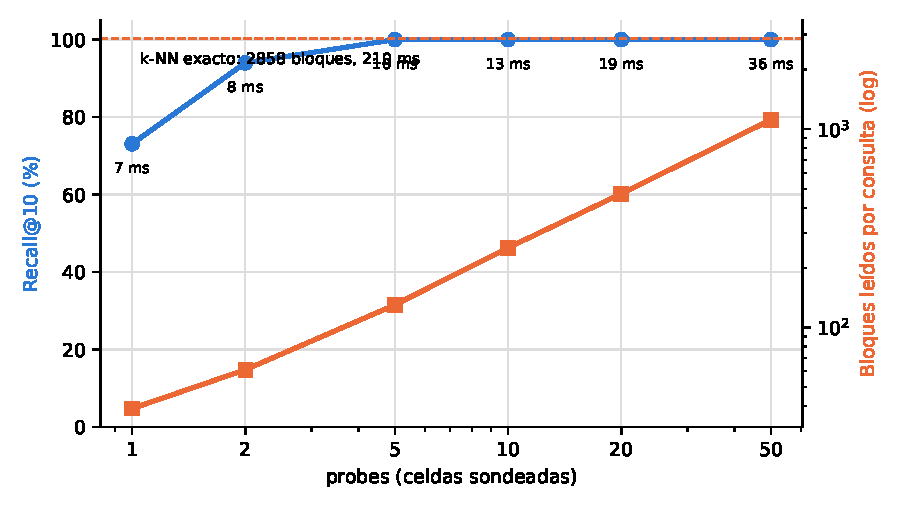
\includegraphics[width=0.78\textwidth]{exp8_recall}
\caption{Curva de compromiso del IVF: el recall crece con \code{probes} mientras los bloques leídos crecen linealmente; con 5 celdas se alcanza recall 1 leyendo 22 veces menos bloques que el escaneo completo.}
\end{figure}

Con una sola celda el IVF ya recupera el 73\,\% de los vecinos verdaderos leyendo
39 bloques frente a los 2858 del escaneo (73 veces menos); con 5 celdas el recall es
1,0 y el costo sigue 22 veces por debajo. A partir de ahí sondear más celdas solo
suma I/O: la curva es la ``rodilla'' clásica del Recall vs.\ costo y justifica el
valor por defecto \code{ivf.probes = 5}. Las 10 lecturas de tabla son constantes
(una página por cada uno de los $k$ resultados), así que todo el costo variable es
del índice.

\begin{table}[H]
\centering\small
\begin{tabular}{rllrrrr}
\toprule
Selectividad & Estrategia & Recall@10 & ms & bloques & índice / tabla & ampliaciones \\
\midrule
0,1\,\% & PRE & 1,00 & 5,0 & 23 & 2 / 21 & 0 \\
0,1\,\% & POST & 0,95 & 3410,4 & 14126,6 & 2407 / 11719 & 3,6 \\
1\,\% & PRE & 1,00 & 8,1 & 204 & 3 / 201 & 0 \\
1\,\% & POST & 0,88 & 281,9 & 1332,8 & 284 / 1048 & 0,65 \\
5\,\% & PRE & 1,00 & 35,3 & 1009 & 8 / 1001 & 0 \\
5\,\% & POST & 1,00 & 83,2 & 333,1 & 126 / 207 & 0 \\
25\,\% & PRE & 1,00 & 126,0 & 5032 & 31 / 5001 & 0 \\
25\,\% & POST & 1,00 & 17,8 & 165,4 & 126 / 39 & 0 \\
100\,\% & PRE & 1,00 & 457,1 & 20124 & 124 / 20000 & 0 \\
100\,\% & POST & 1,00 & 9,9 & 136,3 & 126 / 10 & 0 \\
\bottomrule
\end{tabular}
\caption{Experimento 8b (\code{exp8\_hibrido.csv}): pre- vs.\ post-filtrado con B+ sobre \code{precio} e IVF con 5 probes, forzando la estrategia con \code{SET hybrid.strategy}.}
\end{table}

\begin{figure}[H]
\centering
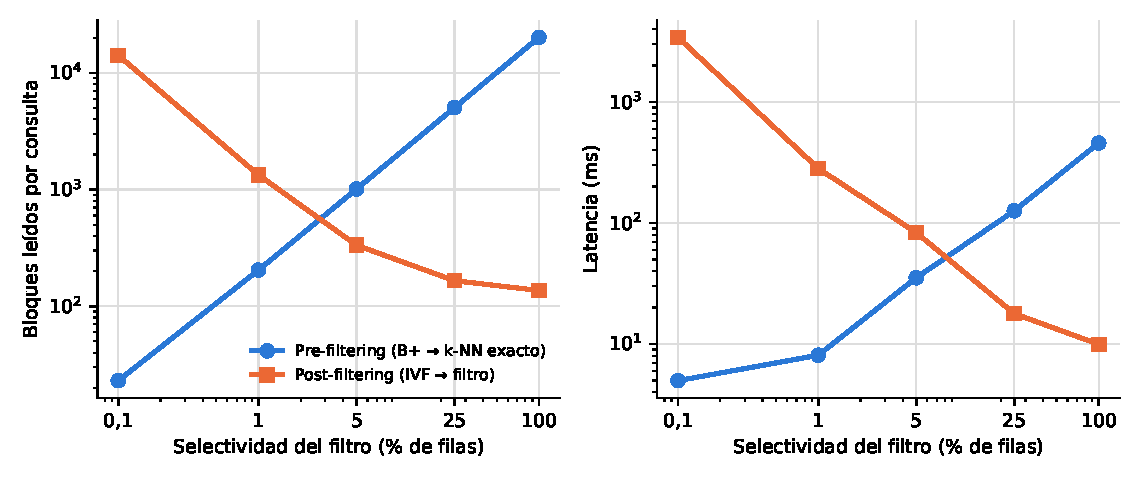
\includegraphics[width=0.95\textwidth]{exp8_hibrido}
\caption{Costo de PRE y POST según la selectividad del filtro. Las curvas se cruzan entre el 1\,\% y el 5\,\%: ahí cambia la decisión del planificador.}
\end{figure}

El cruce está entre 1\,\% y 5\,\% de selectividad. Con filtros muy selectivos el
post-filtrado descarta casi todos los candidatos del IVF y debe ampliar el sondeo
(3,6 veces en promedio al 0,1\,\%), leyendo 600 veces más bloques que el pre-filtrado
y aun así con recall menor que 1; con filtros poco selectivos el pre-filtrado degenera
en un escaneo de la tabla (20\,124 bloques al 100\,\%) mientras el IVF resuelve la
consulta con 136. El estimador del planificador reproduce esta frontera con el conteo
real del índice relacional, que es lo que el Experimento 8b calibra.
